\documentclass[12pt]{article}
\usepackage[margin=1in]{geometry}
\usepackage{amsmath,amssymb}
\usepackage{booktabs,multirow,threeparttable}
\usepackage{graphicx}
\usepackage{natbib}
\usepackage{setspace}
\usepackage[hidelinks]{hyperref}
\usepackage{caption}
\newcommand{\champForecastLL}{0.324}
\newcommand{\champForecastAcc}{86.2}
\newcommand{\champContestedAcc}{85.1}
\newcommand{\champAPRE}{0.48}
\newcommand{\incForecastLL}{0.348}
\newcommand{\champGain}{0.024}
\newcommand{\champCongressoutLL}{0.643}
\newcommand{\majorityCongressoutLL}{0.617}
\newcommand{\gbRawForecastLL}{0.803}
\newcommand{\prospectiveVoneLL}{0.331}
\newcommand{\prospectiveVoneAcc}{85.7}
\newcommand{\prospectiveVtwoLL}{0.332}
\newcommand{\prospectiveVtwoAcc}{86.8}
\newcommand{\prospectiveN}{9,451}
\newcommand{\regimeAbestLL}{0.153}

% auto-generated context
\newcommand{\ukRoll}{1235}
\newcommand{\ukDate}{2024-12-20}
\newcommand{\ukCut}{3.44}
\newcommand{\ukDiscrim}{-1.11}
\newcommand{\ukYeaShare}{92}
\newcommand{\ukNPred}{400}

\newcommand{\revoltProbeR}{0.25}
\newcommand{\revoltProbeN}{944}
\newcommand{\ssfaAUCtext}{0.74}
\newcommand{\ssfaDefectors}{71}
\newcommand{\ssfaAUCnotext}{0.69}

\newcommand{\seenLLchamp}{0.504}
\newcommand{\freshLLchamp}{0.300}
\newcommand{\seenLLnotext}{0.590}
\newcommand{\freshLLnotext}{0.421}
\newcommand{\seenLLclean}{0.518}
\newcommand{\freshLLclean}{0.325}
\newcommand{\seenRC}{368}
\newcommand{\freshRC}{1,911}
\newcommand{\houseLLchamp}{0.306}
\newcommand{\senateLLchamp}{0.464}
\newcommand{\houseLLnotext}{0.434}
\newcommand{\senateLLnotext}{0.480}

\newcommand{\ablOrigLL}{0.328}
\newcommand{\ablOrigAUC}{0.78}
\newcommand{\ablShuffLL}{0.392}
\newcommand{\ablShuffAUC}{0.78}
\newcommand{\ablNoSumLL}{0.351}
\newcommand{\ablNoQLL}{0.383}
\newcommand{\ablNoPropLL}{0.339}
\newcommand{\ablGenTitleLL}{0.340}
\newcommand{\ablRC}{1,957}

\newcommand{\brierChamp}{0.099}
\newcommand{\eceChamp}{0.017}
\newcommand{\defShareRChamp}{0.34}
\newcommand{\brierClean}{0.107}
\newcommand{\eceClean}{0.021}
\newcommand{\defShareRClean}{0.32}
\newcommand{\brierNotext}{0.147}
\newcommand{\eceNotext}{0.028}
\newcommand{\defShareRNotext}{0.27}
\newcommand{\defShareNrc}{995}

\newcommand{\overlapRho}{0.05}
\newcommand{\overlapN}{659}
\newcommand{\paulDefGainPct}{77}
\newcommand{\amashDefGainPct}{73}

\newcommand{\cfAraOrig}{6.5}
\newcommand{\cfAraGeneric}{2.7}
\newcommand{\cfAraPassage}{13.5}
\newcommand{\cfAraBio}{8.4}
\newcommand{\cfArdaOrig}{14.5}
\newcommand{\cfArdaCut}{14.7}
\newcommand{\cfArdaGeneric}{12.6}
\newcommand{\cfArdaSwap}{7.3}

\newcommand{\cutHiDiscR}{0.70}
\newcommand{\cutHiDiscMAE}{0.35}
\newcommand{\cutPassageR}{0.61}
\newcommand{\cutPassageMAE}{0.82}

\newcommand{\paulHeldoutN}{949}
\newcommand{\amashHeldoutN}{579}

\newcommand{\covsummaryChamp}{0.327}
\newcommand{\covtitleonlyChamp}{0.286}
\newcommand{\covdesconlyChamp}{0.370}
\newcommand{\covsummaryNotext}{0.444}
\newcommand{\covtitleonlyNotext}{0.439}
\newcommand{\covdesconlyNotext}{0.377}

\newcommand{\omarDefections}{12}
\newcommand{\omarPctChamp}{92}
\newcommand{\omarPctNotext}{93}
\newcommand{\tlaibDefections}{17}
\newcommand{\tlaibPctChamp}{96}
\newcommand{\tlaibPctNotext}{95}
\newcommand{\bushDefections}{9}
\newcommand{\bushPctChamp}{99}
\newcommand{\bushPctNotext}{92}
\newcommand{\aocDefections}{15}
\newcommand{\aocPctChamp}{93}
\newcommand{\aocPctNotext}{94}
\newcommand{\massieDefections}{177}
\newcommand{\massiePctChamp}{99}
\newcommand{\massiePctNotext}{98}
\newcommand{\royCDefections}{87}
\newcommand{\royCPctChamp}{99}
\newcommand{\royCPctNotext}{97}


\title{Reading the Bills: What Language Models Add\\ to the Measurement of Congress}
\author{Andrew B.\ Hall\thanks{Stanford University. Replication materials,
including the full pipeline, model registry, pre-registered experiment
ledger, and session logs of the AI-assisted development process, are
available in the project repository. Every statistic in this paper is
generated programmatically from analysis output files; none is
transcribed by hand.}}
\date{July 2026}

\begin{document}
\maketitle
\onehalfspacing

\begin{abstract}
\noindent The models political science uses to measure Congress predict
rollcall votes without reading the bills. I build a benchmark of 10.6
million voting decisions (101st--119th Congresses) and a forecasting
model whose language-model encoder takes each bill's pre-vote text as
input, replacing the classical model's free rollcall parameters with
parameters computed from that text. On strictly future votes the model
reaches \champForecastAcc\% accuracy, and a hash-pinned frozen copy
sustains its performance on votes cast after it was frozen. Reading the
bill raises within-vote detection of majority-party defections from
\protAUCnotext{} to \protAUCtext{} AUC, and text plus pre-vote metadata
predicts where a bill will divide the chamber at $r = \cutComboR$ before
anyone votes. Redaction and counterfactual-edit experiments trace the
signal to bill-specific content and procedural posture.
\end{abstract}

\section{Introduction}

On December 20, 2024, the House passed the American Relief Act 366--34,
averting a government shutdown over the objection of 34 Republicans. The
canonical measurement models of political science treat that
rollcall---like every rollcall---as an indexed event with free
parameters estimated from its own votes
\citep{poole1997congress, clinton2004statistical}. The bill itself, the
thing members were reacting to, never enters. As a description of fit
this works remarkably well. But it has two costs. The models are silent
before a vote occurs, because the parameters that would speak do not yet
exist. And when a member defects for a reason one latent dimension
cannot hold---a protest vote, a procedural objection---the model
misplaces the member or writes the vote off as noise.

This paper asks what modern language models add to the measurement of
Congress, and answers by construction: I replace the free rollcall
parameters with parameters \emph{computed from the bill's pre-vote
text}, so that any bill---including one not yet voted on---receives a
predicted cutpoint and a member-by-member forecast. On a benchmark of
10.6 million individual voting decisions from the 101st through 119th
Congresses, the resulting model predicts \champForecastAcc\% of strictly
future votes correctly (\champContestedAcc\% on contested votes), at a
log loss of \champForecastLL{} against \memberqForecastLL{} for the
strongest member-history baseline and \constantForecastLL{} for a
constant prediction.

Three concrete results follow. First, the gains are real out-of-sample
gains, not artifacts of iteration. A version of the model frozen and
hash-pinned in June 2026 scored \prospectiveVoneLL{} log loss on the
\prospectiveN{} decisions Congress cast after its data snapshot,
matching its development performance; the temporal holdout results carry
paired rollcall-cluster bootstrap intervals (the model's margin over its
own strongest component is $[\pairedDeltaOneLo, \pairedDeltaOneHi]$ log
loss); and the text advantage is \emph{larger} on the \freshRC{}
held-out rollcalls whose bills were never voted on in training (log loss
\freshLLchamp{} against \freshLLnotext{} without text) than on bills
with prior votes---the model reads new bills rather than remembering old
ones.

Second, reading the bill lets the model see majority-party defections
coming. On the American Relief Act, an identical model without text
prices the vote as routine majority business; the text model recognizes
a bipartisan must-pass package, and its five likeliest defectors in the
chamber all voted nay. Across \protRC{} held-out majority-side rollcalls
with at least three defections, text raises within-vote defection
detection from \protAUCnotext{} to \protAUCtext{} AUC---about a fifth of
the remaining ranking errors. I trace where this signal lives by feeding
the frozen model corrupted versions of its own inputs: substituting a
different same-topic bill's text costs more than deleting the text
outright ($\ablOrigLL \rightarrow \ablShuffLL$ versus $\ablNoSumLL$ log
loss), so the model uses bill-specific content, not topic membership;
removing the procedural question costs the most
($\ablNoQLL$); and stripping digits costs nothing. Counterfactual edits
on single bills point the same way: replacing the Relief Act's title
with generic language cuts its predicted defection share from
\cfAraOrig\% to \cfAraGeneric\%, while moving the same bill from the
suspension calendar to ordinary passage raises it to \cfAraPassage\%.

Third, text locates bills before anyone votes. Taking each rollcall's
realized cutpoint from standard spatial fits as the target, text plus
pre-vote metadata predicts held-out cutpoints with a mean absolute error
of \cutComboMAE{} member-standard-deviations and a predicted--realized
correlation of $r = \cutComboR$ (no-feature baseline:
\cutConstMAE{} and zero), and classifies which party's side the yeas
fall on for \dirCombo\% of rollcalls against a \dirConst\%
majority-direction baseline. On the half of the holdout where the
target itself is precisely estimated, the correlation rises to
$r = \cutHiDiscR$. The bill-location literature recovers these objects
from realized votes \citep{peress2013estimating, richman2011parties};
here they exist before the vote.

A long line of work anticipates the attempt.
\citet{clinton2004statistical} put ideal-point estimation on a
statistical footing, and a decade of scaling research then built
purpose-built models for the members the workhorse mis-measures:
heteroskedastic ``unpredictable voter'' terms
\citep{lauderdale2010unpredictable}, issue-specific dimensions
\citep{lauderdale2014scaling}, estimators for enormous vote matrices
\citep{imai2016fast}, non-monotone response functions for extremists who
vote with the opposite pole \citep{duckmayr2023ends}, and mixture models
for majority members who cast protest votes against bills they prefer
\citep{fowler2026protest}. A separate program tried to bring text in
with the tools of its era: \citet{gerrish2011predicting} regressed
rollcall parameters on topic models, and \citet{kraft2016embedding}
learned bilinear interactions between member embeddings and word
vectors. That program stalled---reimplemented on this benchmark and
evaluated under proper scoring, neither approach improves on a simple
table of member voting rates (Table~\ref{tab:regime})---and it stalled,
I argue, for two reasons: the encoders of 2011--2016 could not read
legislative language well, and no evaluation discipline separated
genuine forecasting from in-sample curve fitting.

This paper's contribution is threefold. I supply the missing
evaluation infrastructure: an open benchmark with deterministic,
content-hashed splits, a per-field feature-timing audit, a
pre-registered experiment ledger recording negative results, and a
prospective protocol in the spirit of \citet{dwork2015holdout} that
scores frozen artifacts only on votes cast after freezing. I supply the
model: a two-tower architecture that amortizes rollcall parameters from
frozen sentence-encoder embeddings, anchors on member voting histories,
and strictly nests the bilinear model of \citet{kraft2016embedding} as a
special case---so the comparison isolates what each added part buys. And
I supply new measurement objects the classical toolkit cannot produce:
pre-vote defection risks that anticipate the protest voting
\citet{fowler2026protest} can only reinterpret after the fact, and
pre-vote bill locations. The same experiments map where the method
stops: text adds little in the Senate, member histories fail at House
majority transitions, and amendment language carries no signal beyond
the amending actor's party.

Section~\ref{sec:data} describes the panel, the text inputs and their
timing rules, and the evaluation protocol. Section~\ref{sec:models}
presents the models, from the classical spatial benchmark through the
two-tower architecture, and states exactly how each relates to its
predecessors. Section~\ref{sec:results} reports the forecasting horse
race, the member-level fit comparison, the defection results with the
redaction experiments, and the cutpoint predictions.
Section~\ref{sec:limits} reports three measured boundaries, and
Section~\ref{sec:conclusion} concludes with two concrete extensions.

\section{Data, Benchmark, and Protocol}
\label{sec:data}

The panel is every recorded yea or nay by every member of the House and
Senate in the 101st through 119th Congresses---10.6 million
member--vote decisions on roughly 27,000 rollcalls---from Voteview
\citep{lewis2026voteview}. The unit of analysis is the member--rollcall
cell $(i,v)$ with outcome $y_{iv} \in \{0,1\}$; abstentions and
absences are excluded. Bill-side information comes from the government's
BILLSTATUS files, which begin with the 108th Congress: titles, sponsors,
policy areas, and dated summary versions. All text-based results
therefore use the 108th--119th Congresses.

\paragraph{Text inputs and timing.} For each rollcall I assemble the
text a contemporaneous observer could have read: the Clerk's vote
question, the vote description, and the latest Congressional Research
Service summary whose action date falls \emph{strictly before} the vote
date, with the bill title as fallback. A frozen sentence encoder
(all-MiniLM-L6-v2, 384 dimensions) embeds the first 1,500 characters; a
second encoder (Qwen3-Embedding, 1,024 dimensions) embeds 6,000
characters. Two fields are generated at the vote itself and admit no
earlier timestamp---the question and description---and the redaction
experiments of Section~\ref{sec:defections} bound their contribution.
One ensemble component also uses CRS-curated subject terms, which are
revisable without version history; every headline number therefore
appears twice, once for the full ensemble and once for the single tower
whose inputs are fully leakage-clean.

\paragraph{Evaluation regimes.} Four regimes impose progressively
stricter information constraints. \emph{Completion} holds out random
member--vote cells by a salted SHA-256 hash, leaving same-rollcall votes
observable---the psychometric setting in which ideal-point models are
traditionally assessed. \emph{Temporal forecast}, the primary regime,
holds out the final 10\% of each congress-chamber's rollcalls by date.
\emph{Congress-out} trains through the 116th Congress, validates on the
117th, and tests on the 118th. \emph{Prospective} scores hash-pinned
frozen artifacts only on votes cast after their data snapshot. Metrics
are the field's: correct classification, aggregate proportional
reduction in error (APRE), and geometric mean probability
\citep{carroll2013structure}, with log loss as the primary scoring
rule; within-vote defection detection uses the area under the ROC curve
(AUC) computed per rollcall and averaged with equal weight.

\paragraph{Protocol.} Development followed a pre-registered experiment
ledger: hypothesis, a statement of why the information should be
knowable pre-vote, and a falsification criterion, all recorded before
each experiment's first run. Model selection used validation sets only;
the final model comparison observed test sets once. Negative results
are retained and reported. The evaluation harness strips labels before
models see evaluation rows, and the replication package regenerates
every exhibit from raw files in under two GPU-hours on a laptop-class
accelerator.

\section{Models}
\label{sec:models}

\subsection{The classical benchmark, made competitive}
\label{sec:spatial}

The workhorse spatial model says member $i$ votes yea on rollcall $v$
with probability
\begin{equation}
\Pr(y_{iv}=1) \;=\; \sigma\!\left(\mathbf{a}_v^\top \mathbf{x}_i + b_v
+ c_i\right),
\label{eq:irt}
\end{equation}
where $\mathbf{x}_i \in \mathbb{R}^k$ is the member's position, $c_i$
is a member intercept capturing base yea-propensity,
$\mathbf{a}_v \in \mathbb{R}^k$ and $b_v$ are the rollcall's
discrimination and difficulty, and $\sigma$ is the logistic function.
With $k=1$ and $c_i = 0$, equation~(\ref{eq:irt}) is exactly the
two-parameter model of \citet{clinton2004statistical}; the intercept
and higher dimensions are strict generalizations. I estimate it by
minibatch AdamW (learning rate .05, weight decay $10^{-4}$, batch
$2^{17}$), with weight decay playing the role of the Bayesian prior and
early stopping on an internal 2\% slice of training data. Dimension one
is seeded at $\pm 0.5$ by party, which fixes the orientation of the
learned axis without constraining what the data can express. The
classical reference point, \textsc{NominateLogit}, freezes positions at
two-dimensional DW-NOMINATE scores and estimates only
$(\mathbf{a}_v, b_v)$, by the same optimizer on the same cells---so
every comparison between the two isolates what flexible positions add
under an identical likelihood.

\subsection{The two-tower text model}
\label{sec:tower}

The forecasting model replaces the free rollcall parameters of
(\ref{eq:irt}) with parameters \emph{amortized} from pre-vote features:
\begin{equation}
\operatorname{logit}\Pr(y_{iv}=1) \;=\;
g_a(\phi_v)^\top \mathbf{x}_i \;+\; g_b(\phi_v) \;+\; c_i \;+\;
\boldsymbol\gamma^\top \mathbf{z}_{iv}.
\label{eq:tower}
\end{equation}
Here $\phi_v$ concatenates the rollcall's sentence embedding with
question-bucket, bill-category, and sponsor-party indicators; the heads
$g_a: \mathbb{R}^d \to \mathbb{R}^{16}$ and
$g_b: \mathbb{R}^d \to \mathbb{R}$ are two-layer perceptrons (width
128) mapping features to discrimination and difficulty; and
$\mathbf{z}_{iv}$ holds member--rollcall covariates: indicators for
sharing or opposing the sponsor's party, plus the logit of member $i$'s
empirical yea rate in the vote's question bucket. That last term
deserves emphasis. The member-history rate enters as an offset with a
learned weight $\gamma$ initialized at one, so the network starts from
``trust the count table'' and must earn any departure---and the count
table turns out to be the binding baseline that the earlier text
literature never cleared.

Because the amortization heads take text as input, a bill the model has
never seen receives a discrimination vector, a difficulty, and hence a
predicted cutpoint and member-by-member forecast. That single design
choice produces every prospective capability in the paper.

Training uses AdamW (learning rate .02, weight decay $10^{-4}$, batch
$2^{17}$) with early stopping and post-hoc temperature calibration on a
\emph{temporal} internal slice---the final 5\% of training rollcalls by
date, whole rollcalls, strictly inside the training window. A
random-cell slice is in-sample for rollcall parameters and miscalibrates
forecasts; the temporal slice sees future-like data. The final model is
a logistic blend, fit on the same slice, of three towers that differ
only in text representation: the MiniLM tower (blend weight 0.57), a
TF--IDF tower over title, policy area, and subjects (0.12), and the
Qwen tower (0.42). The no-text counterfactual used throughout deletes
the embedding block and keeps everything else, independently trained and
calibrated---nothing is inherited from text models.

\subsection{Relation to existing models}
\label{sec:relation}

Equation~(\ref{eq:tower}) nests the bilinear model of
\citet{kraft2016embedding}: set the heads linear, drop the metadata
blocks from $\phi_v$, and drop $\mathbf{z}_{iv}$, and what remains is
their member-embedding-times-text-embedding core. My reimplementation
of that special case, given modern sentence embeddings and matched
capacity, scores \kraftForecastLL{} log loss on the temporal
holdout---behind the \memberqForecastLL{} count table. The
\citet{gerrish2011predicting} design regresses the parameters of
(\ref{eq:irt}) on text after fitting; my two-stage reimplementation
scores \gbRawForecastLL{} as published (worse than a constant
prediction, because it is uncalibrated) and \gbTcalForecastLL{} with
temperature calibration added. The additions that matter, in the order
the experiment ledger established them, are the member-history offset,
the temporal development slice with calibration, and the nonlinear
heads. Relative to structured item-response theory, the distinctive
commitments are pre-vote-only text, frozen encoders (fine-tuning was
tested and rejected), and the evaluation protocol.

\section{Results}
\label{sec:results}

\subsection{The forecasting horse race}

Table~\ref{tab:regime} reports the temporal-forecast comparison: every
model predicts the final 10\% of each congress-chamber's rollcalls from
the preceding 90\%. The blend reaches \champForecastLL{} log loss
(\champForecastAcc\% accuracy, \champContestedAcc\% on contested votes,
APRE \champAPRE) on \forecastTestN{} future votes; the leakage-clean
single tower reaches \incForecastLL. The member-history count table, at
\memberqForecastLL, beats every 2011--2016 text architecture, which is
the quantitative sense in which the earlier program stalled. The paired
bootstrap margin of the blend over its strongest component,
$[\pairedDeltaOneLo, \pairedDeltaOneHi]$ log loss, is small; the margin
over the no-text counterpart, \notextForecastLL{} to \champForecastLL,
is not. Predicted probabilities are usable as probabilities: expected
calibration error is \eceChamp{} (Brier \brierChamp) against
\eceNotext{} without text.

\begin{table}[tbp]
\centering
\begin{threeparttable}
\caption{Temporal-forecast comparison. Each model predicts the final
10\% of each congress-chamber's rollcalls (108th--119th Congresses)
from the preceding 90\%; identical evaluation cells throughout. The
right panel reports transfer to a fully held-out congress
(Section~\ref{sec:limits}).}
\label{tab:regime}
\begin{tabular}{lcccc}
\toprule
Information used & \multicolumn{2}{c}{Temporal forecast} & \multicolumn{2}{c}{Congress-out} \\
\midrule
Party history only & 0.466 & 76.6 & 0.693 & 57.1 \\
Member history only & 0.459 & 76.0 & 0.693 & 57.1 \\
Rollcall metadata only & 0.511 & 72.3 & 0.717 & 58.6 \\
Text + metadata (no member history) & 0.464 & 77.8 & 0.741 & 64.4 \\
Text + metadata + member history & 0.411 & 80.1 & 0.720 & 59.3 \\
+ modern encoder, deep head, calibration & 0.348 & 85.2 & 0.670 & 61.6 \\
+ ensemble (final) & 0.324 & 86.2 & 0.643 & 62.1 \\
\bottomrule
\end{tabular}

\end{threeparttable}
\end{table}

Two audits discipline these numbers. Table~\ref{tab:prospective} scores
the frozen artifacts: the June 12, 2026 freeze recorded
\prospectiveVoneLL{} log loss (\prospectiveVoneAcc\% accuracy) on the
\prospectiveN{} member-votes cast after its data snapshot, and
\postFreezeLL{} on the strictly post-freeze subset---consistent with
development performance, though the cluster count (\prospectiveRC{}
rollcalls) keeps this audit preliminary. And the seen/fresh split rules
out bill-family memorization: the text gain is larger on fresh bills
(\freshLLchamp{} versus \freshLLnotext) than on bills with prior
training-window votes (\seenLLchamp{} versus \seenLLnotext).

\begin{table}[tbp]
\centering
\begin{threeparttable}
\caption{Prospective audit. Hash-pinned artifacts are scored only on
votes cast after their June 9, 2026 data snapshot; the rollcall-cluster
bootstrap 95\% interval for the v1 log loss is
\prospLLlo--\prospLLhi.}
\label{tab:prospective}
\begin{tabular}{llrrccc}
\toprule
Artifact & Snapshot & Rollcalls & Votes & Log loss & Acc.\ (\%) & AUC \\
\midrule
v1 (emb2-MLP tower) & 2026-06-09 & 43 & 9,451 & 0.331 & 85.7 & 0.924 \\
v2 (three-tower blend) & 2026-06-09 & 43 & 9,451 & 0.332 & 86.8 & 0.921 \\
\bottomrule
\end{tabular}

\end{threeparttable}
\end{table}

\subsection{Member-level fit against the canonical measure}
\label{sec:fit}

The completion regime asks the classical question: how well does a
spatial model fit held-out votes when same-rollcall votes remain
observable? No text enters here; the comparison isolates model
flexibility. Figure~\ref{fig:membercc} plots each member's percent of
held-out votes correctly classified under the eight-dimensional model
of Section~\ref{sec:spatial} against \textsc{NominateLogit}, on
identical cells that neither model's parameters saw. The median member
is classified correctly \memberCCmedNom\% of the time by the classical
model and \memberCCmedOurs\% by the flexible one---for the typical
member, DW-NOMINATE is nearly unimprovable. The flexible model is more
accurate for \memberCCshare\% of members, and the gains concentrate
exactly where a decade of bespoke scaling models aimed: Ron Paul's
correct-classification rate rises from \paulCCnom\% to \paulCCours\%,
and his largest per-vote improvements are nay votes on defense
authorizations and surveillance reauthorizations that the classical
model priced below two percent. Today's left flank is absent from this
tail for an instructive reason: frozen DW-NOMINATE already classifies
Ilhan Omar at \omarCCnom\% and Rashida Tlaib at \tlaibCCnom\%, because
members at the scale's extreme are easy to classify even when their
individual protest votes are missed. Their measurement story appears in
the next subsection. Convergent validity survives the added
flexibility: first-dimension positions correlate with DW-NOMINATE at
$r=.98$ and with Nokken--Poole per-congress scores
\citep{nokken2004congressional} at $r=\npRmin$--$\npRmax$.

\begin{figure}[tbp]
\centering
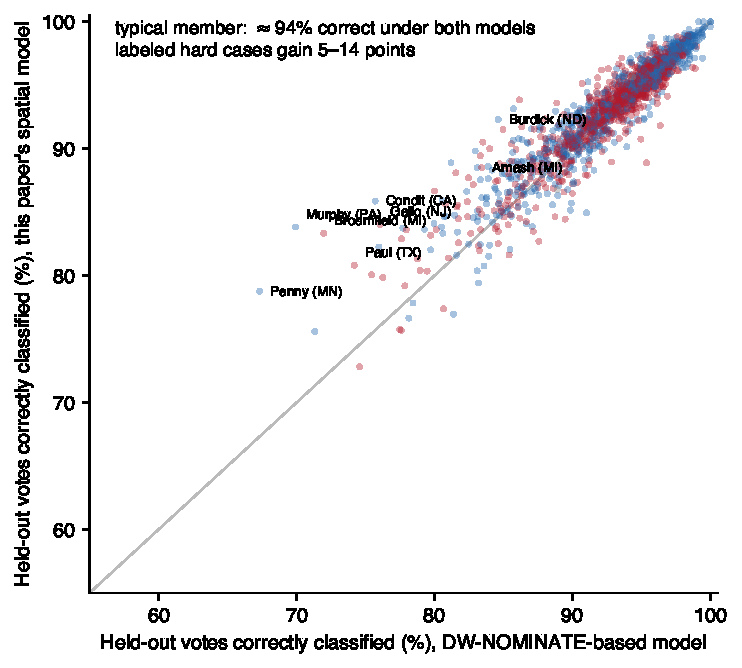
\includegraphics[width=.66\linewidth]{figures/member_cc.pdf}
\caption{Member-level fit on identical held-out votes, completion
regime. Each point is one member with at least 100 held-out votes,
plotting percent correctly classified under the flexible spatial model
(vertical) against the frozen-DW-NOMINATE model (horizontal); blue
marks Democrats, red Republicans. Labeled members have the largest
gains.}
\label{fig:membercc}
\end{figure}

\subsection{Defections before the vote, and where the signal lives}
\label{sec:defections}

Define a defection as a majority-party member voting nay when the
party's majority votes yea. Defections include the protest votes that
are the scaling literature's newest problem
\citep{fowler2026protest, duckmayr2023ends}---treated there
retrospectively, by reinterpreting votes already cast. The forecasting
model prices them in advance. Figure~\ref{fig:protest} shows the
American Relief Act twice: predicted by the no-text counterpart, which
sees a routine majority bill, and by the text model, which moves
Democratic probabilities to near one, slides Republican probabilities
with distance from the center, and ranks Brecheen, Roy, Massie, Crane,
and Biggs as the chamber's five likeliest defectors. All five voted
nay. The bill's pre-vote text was six words of title plus the
suspension-calendar question---which is the point: the model read what
an observer could read the night before, and it sufficed.

\begin{figure}[tbp]
\centering
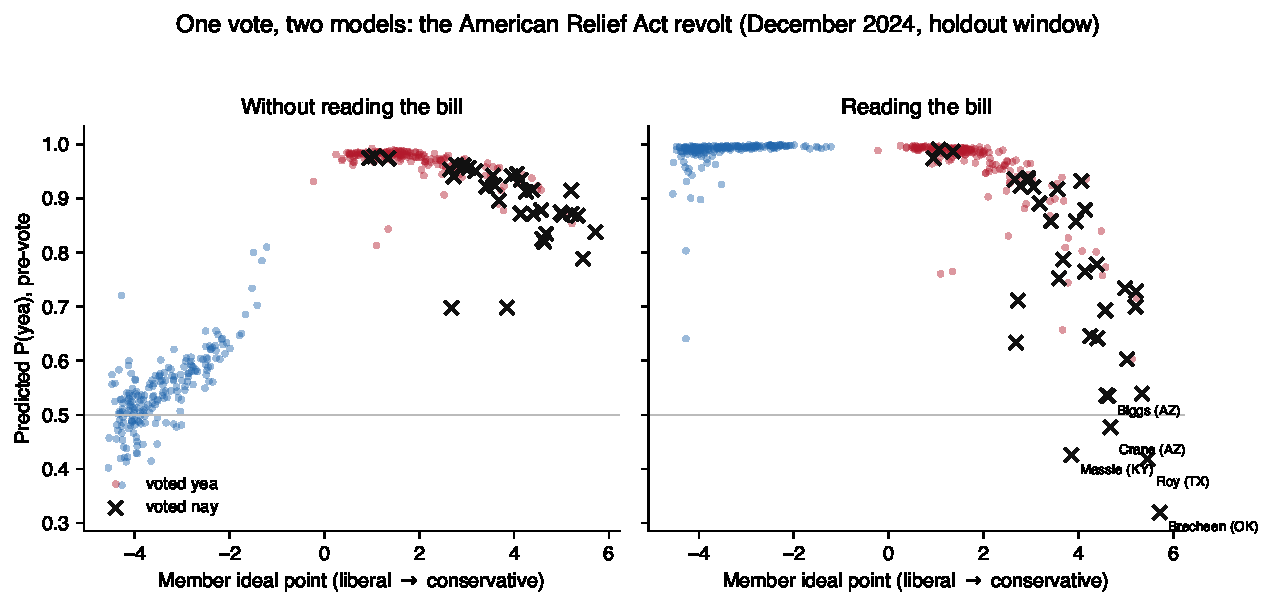
\includegraphics[width=.95\linewidth]{figures/protest_detection.pdf}
\caption{One majority-splitting vote (H.R.~10545, December 20, 2024),
predicted by the same architecture without text (left) and with it
(right). Dots are members who voted yea, colored by party; crosses are
the 34 nays; members are placed by first-dimension ideal point. The
text model's five likeliest defectors chamber-wide, labeled at right,
all voted nay.}
\label{fig:protest}
\end{figure}

Figure~\ref{fig:capture} pools the episode across all \protRC{}
majority-yea holdout rollcalls with at least three defections
(\protN{} defections). Within-vote AUC rises from \protAUCnotext{}
without text to \protAUCtext{} with it; the fully leakage-clean tower
scores \protAUCclean, so no revisable metadata drives the gain, and the
unfiltered all-defection version gives \protAUCtextAll{} against
\protAUCnotextAll. Panel~(a) shows the gain is a distribution, not a
uniform shift: the text model is higher on 70\% of rollcalls, and the
largest lifts land on the votes member history prices worst. Panel~(b)
translates the statistic: screening majority members in the model's
risk order finds any given share of eventual defectors several members
sooner than the no-text ranking. Member by member
(Table~\ref{tab:defectors}), both flanks are priced well before the
vote: when Thomas Massie or Chip Roy defects, the model has him at the
99th percentile of predicted risk within his party; when Rashida Tlaib
or Cori Bush defects, she sits at the \tlaibPctChamp th and
\bushPctChamp th percentiles. For the left flank the no-text model does
nearly as well---their defections are stable habits---while text
contributes most to the situation-triggered revolts of the right flank.

\begin{figure}[tbp]
\centering
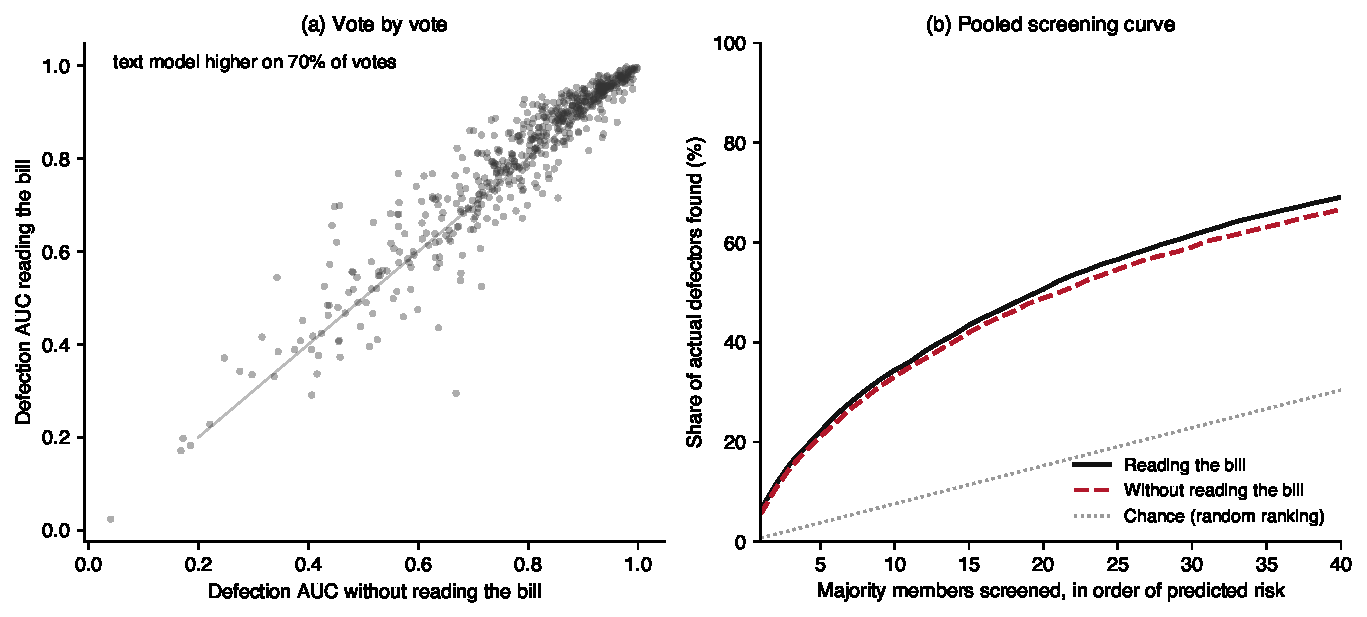
\includegraphics[width=.95\linewidth]{figures/defector_capture.pdf}
\caption{Defection detection pooled across majority-yea holdout
rollcalls with at least three defections. Panel (a): within-vote AUC
computed rollcall by rollcall, text model (vertical) against no-text
counterpart (horizontal). Panel (b): share of actual defectors found
among the top-$k$ majority members ranked by predicted risk, averaged
over rollcalls; the dotted line is a random ranking.}
\label{fig:capture}
\end{figure}

\begin{table}[tbp]
\centering
\begin{threeparttable}
\caption{Habitual majority defectors in the temporal holdout. ``Rate''
is defections per majority-yea passage-family vote in the member's
holdout windows. The risk percentile is the member's mean percentile of
predicted defection probability within their party, computed before
each vote, on the votes where the member in fact defected (100 = ranked
the party's likeliest defector every time).}
\label{tab:defectors}
{\small \begin{tabular}{lcccc}
\toprule
 & & & \multicolumn{2}{c}{Mean pre-vote risk percentile} \\
\cmidrule(lr){4-5}
Member & Defections & Rate & Text model & No-text \\
\midrule
\multicolumn{5}{l}{\emph{Republican majorities (top 8 by defection rate)}} \\
\quad Rosendale (R-MT) & 71 & 56\% & 97 & 96 \\
\quad Roy (R-TX) & 87 & 52\% & 99 & 97 \\
\quad Good (R-VA) & 63 & 48\% & 93 & 92 \\
\quad Paul (R-TX) & 103 & 48\% & 99 & 99 \\
\quad Biggs (R-AZ) & 120 & 46\% & 98 & 97 \\
\quad Greene (R-GA) & 51 & 45\% & 97 & 95 \\
\quad Massie (R-KY) & 177 & 42\% & 99 & 98 \\
\quad Amash (R-MI) & 122 & 41\% & 98 & 98 \\
\multicolumn{5}{l}{\emph{Democratic majorities (top 8 by defection rate)}} \\
\quad Bright (D-AL) & 22 & 35\% & 99 & 98 \\
\quad Feingold (D-WI) & 19 & 26\% & 89 & 92 \\
\quad Adler (D-NJ) & 17 & 24\% & 91 & 95 \\
\quad Minnick (D-ID) & 16 & 23\% & 99 & 99 \\
\quad Shuler (D-NC) & 38 & 22\% & 94 & 94 \\
\quad Nye (D-VA) & 15 & 19\% & 96 & 93 \\
\quad Byrd (D-WV) & 9 & 19\% & 81 & 82 \\
\quad Kratovil (D-MD) & 14 & 18\% & 97 & 99 \\
\multicolumn{5}{l}{\emph{The modern left flank (named cases; 116th--117th windows)}} \\
\quad Tlaib (D-MI) & 17 & 9\% & 96 & 95 \\
\quad Ocasio-Cortez (D-NY) & 15 & 8\% & 93 & 94 \\
\quad Bush (D-MO) & 9 & 8\% & 99 & 92 \\
\quad Omar (D-MN) & 12 & 6\% & 92 & 93 \\
\quad Pressley (D-MA) & 11 & 6\% & 93 & 93 \\
\bottomrule
\end{tabular}
}
\end{threeparttable}
\end{table}

Where in the text does the signal live? Table~\ref{tab:ablation}
re-scores the frozen model on all \ablRC{} legislation-linked holdout
rollcalls after corrupting one input at a time; every non-text feature
is held fixed, so differences isolate the text component. Three
findings structure the table. Removing the vote question costs the most
($\ablOrigLL \rightarrow \ablNoQLL$): the procedural posture of a vote
is the single most informative phrase the model reads. The placebo is
the sharpest test: replacing a bill's text with a \emph{different}
bill's from the same policy area and question type costs
$\ablShuffLL$---more than deleting the text outright
($\ablNoSumLL$)---so topic-matched but wrong-bill text actively
misleads, and the model must be using bill-specific content. And
masking proper nouns costs little ($\ablNoPropLL$) while stripping
digits costs nothing: the model does not run on names and dates.
Replacing every title with generic language costs \ablGenTitleLL,
pooling across the corpus the single-bill title effect above. A linear
probe makes the same point without any member data: ridge-regressing
each rollcall's majority-defection share on its text embedding alone
predicts held-out defection shares at $r=\revoltProbeR$ across
\revoltProbeN{} majority-side votes.

\begin{table}[tbp]
\centering
\begin{threeparttable}
\caption{Redaction experiments. Each row feeds the frozen model a
corrupted version of the exact text template it was trained on, for all
\ablRC{} legislation-linked holdout rollcalls, holding every non-text
input fixed; the defection AUC column is the noisier statistic (507
rollcalls) and log loss is the scoring rule.}
\label{tab:ablation}
{\small \begin{tabular}{lccc}
\toprule
Text given to the frozen model & Log loss & $\Delta$ & Defection AUC \\
\midrule
Original text & 0.328 &  & 0.784 \\
Bill summary removed & 0.351 & +0.023 & 0.811 \\
Vote question removed & 0.383 & +0.055 & 0.766 \\
Titles replaced by generic language & 0.340 & +0.012 & 0.768 \\
Proper nouns masked & 0.339 & +0.011 & 0.779 \\
Digits removed & 0.328 & +0.000 & 0.787 \\
Text from another bill, same policy area & 0.392 & +0.064 & 0.777 \\
\bottomrule
\end{tabular}
}
\end{threeparttable}
\end{table}

Text similarity is not the whole mechanism, and one failure shows the
seam. The Social Security Fairness Act drew a 34\% majority defection,
yet its nearest neighbors in embedding space are consensual benefit
expansions that drew almost none---the conflict was procedural (the
bill reached the floor by discharge petition), and nothing in the
summary's language marks it. The full model still ranks its
\ssfaDefectors{} Republican defectors better than the no-text twin
(within-vote AUC \ssfaAUCtext{} against \ssfaAUCnotext), drawing on
member history and institutional features. The division of labor is:
text locates a bill among its substantive precedents, procedural
posture signals how contested the leadership expects the vote to be,
and member history supplies who sits where.

\subsection{Where a bill will divide the chamber}
\label{sec:cutpoints}

If bill content organizes coalitions, a bill's text should locate it
before anyone votes. I take each rollcall's \emph{realized cutpoint}
$x_v^* = -(b_v + \bar c)/a_v$ and direction $\mathrm{sign}(a_v)$ from
one-dimensional per-chamber-congress fits of (\ref{eq:irt}) on all
votes, standardized within chamber-congress and reported when
$|a_v| \ge 0.35$; this is a property of the realized vote, not the
proposal or status-quo location of \citet{peress2013estimating}. Within
each congress-chamber the first 80\% of rollcalls train ridge (location)
and logistic (direction) predictors on strictly pre-vote features, and
the final 20\% are held out.

Figure~\ref{fig:cutpred} and Table~\ref{tab:cutpred} give the result on
the \cutTestN{} identified held-out rollcalls. Text plus metadata
reaches a mean absolute error of \cutComboMAE{}
member-standard-deviations and $r = \cutComboR$, against \cutConstMAE{}
and zero for the no-feature baseline, and calls direction for
\dirCombo\% of rollcalls against the \dirConst\% majority-direction
baseline. Institutional metadata alone---question type, sponsor party,
and on amendment votes the amender's party---is a strong start
(\cutMetaMAE, \dirMeta\%), which is what majority agenda control
implies; text improves every margin beyond it, most of all direction.
Because the target is itself an estimate, precision strata matter: on
the high-discrimination half of the holdout, where realized cutpoints
are pinned tightly, the error falls to \cutHiDiscMAE{} and the
correlation rises to $r = \cutHiDiscR$---much of the headline error is
noise in the target, not the prediction. At the term level, the
language of program-building (\emph{establish}, \emph{grants},
\emph{assistance}) predicts liberal-yea coalitions and the language of
restraint (\emph{rule}, \emph{regulation}, \emph{permit}) predicts
conservative-yea ones; these are predictive associations on a curated
agenda, not causal claims about language.

\begin{figure}[tbp]
\centering
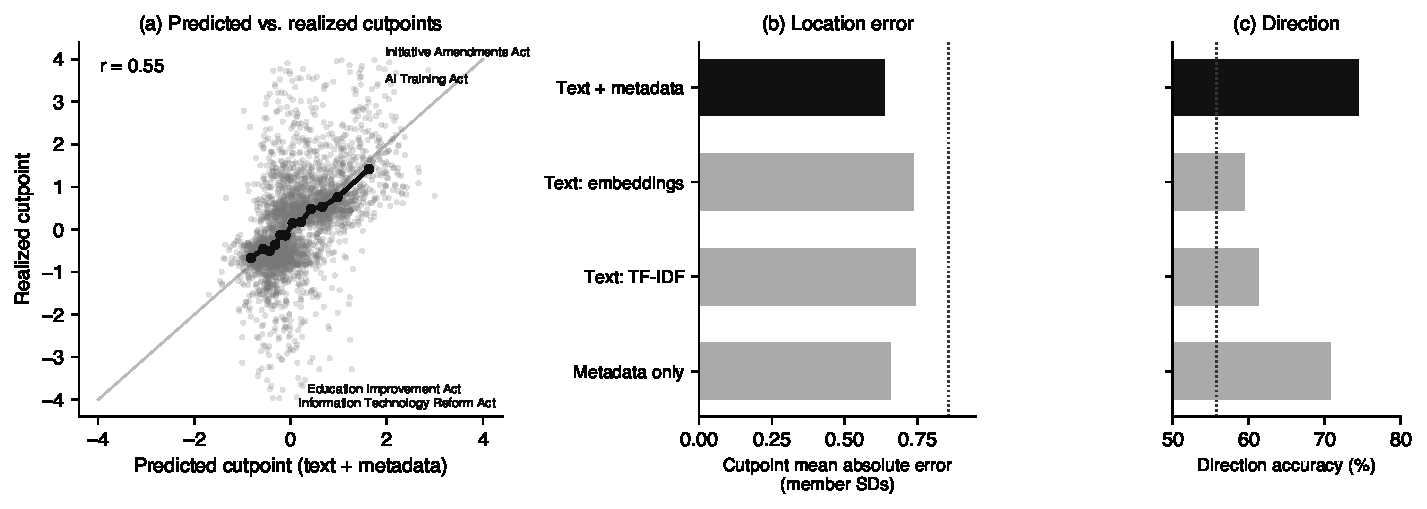
\includegraphics[width=.95\linewidth]{figures/cutpoint_prediction.pdf}
\caption{Predicting held-out rollcalls' cutpoints from pre-vote
features. Panel (a): predicted (horizontal) against realized (vertical)
cutpoints under the text-plus-metadata model, in
member-standard-deviation units; the black line connects binned means
and the gray line is the diagonal. Panels (b) and (c): location error
and direction accuracy by feature set, with the full model in black and
dotted lines marking the no-feature and majority-direction baselines.}
\label{fig:cutpred}
\end{figure}

\begin{table}[tbp]
\centering
\begin{threeparttable}
\caption{Cutpoint and direction prediction by feature set, held-out
rollcalls. The bottom panel decomposes the text input by component.}
\label{tab:cutpred}
\begin{tabular}{lccc}
\toprule
Features & Cutpoint MAE & Cutpoint $r$ & Direction acc.\ (\%) \\
\midrule
Constant & 0.856 & 0.00 & 55.8 \\
Metadata only & 0.657 & 0.48 & 70.8 \\
Text: TF--IDF & 0.742 & 0.43 & 61.3 \\
Text: embeddings & 0.735 & 0.42 & 59.5 \\
Text + metadata & 0.637 & 0.55 & 74.5 \\
\quad question only & 0.763 & 0.41 & 58.2 \\
\quad description only & 0.813 & 0.25 & 57.2 \\
\quad bill summary only & 0.765 & 0.38 & 59.7 \\
\bottomrule
\end{tabular}

\end{threeparttable}
\end{table}

The prediction is also a usable index. Computed over the 118th House's
final months, the predicted majority-defection share sorts the agenda
by revolt risk before any votes are cast; its largest predicted risks
and the window's largest realized revolts are the same kind of
bill---continuing resolutions and lands-, recognition-, and
commemoration-type spending items. Party unity rates and roll rates
summarize stress on party government after the votes; this index prices
each agenda item as it arrives.

\section{Three Measured Boundaries}
\label{sec:limits}

The same infrastructure that certifies the gains maps their limits, and
all three boundaries are measured rather than conjectured.

\emph{The Senate.} The text gain concentrates in the House
(\houseLLchamp{} against \houseLLnotext{} without text; defection AUC
\protAUCtextHouse{} against \protAUCnotextHouse) and nearly vanishes in
the Senate (\senateLLchamp{} against \senateLLnotext; AUC
\protAUCtextSenate{} against \protAUCnotextSenate{} over
\protRCsenate{} rollcalls). Where floor access is negotiated vote by
vote, the marginal information in a bill's text is small.

\emph{Majority transitions.} At every House majority flip in the
window---and at no placebo transition---the procedural component of
member history stops transferring: procedural log loss averages
\flipProcLL{} across flips against \placeboProcLL{} across placebos,
while final-passage transfer is flip-invariant (\flipPassLL{} against
\placeboPassLL). Procedural voting records institutional role, not
stable preference, and scores estimated in one majority configuration
should cross configurations only with care \citep{bateman2017house}.
The congress-out panel of Table~\ref{tab:regime} shows the aggregate
consequence: transfer to a fully held-out congress remains unsolved,
for every model.

\emph{Amendments.} Supplying amendments' purpose text makes prediction
worse, not better, in pre-registered, placebo-controlled experiments;
what moves amendment prediction is the amending actor's party, which
takes direction accuracy from roughly a coin flip to 77\%. Short
purpose text adds nothing once bill identity and procedural context are
modeled.

\section{Conclusion}
\label{sec:conclusion}

The free rollcall parameters of the classical spatial model are both
its strength and its blind spot: they absorb everything, so they
explain nothing in advance. Making those parameters a function of the
bill's pre-vote text converts a fitting device into a forecasting
instrument, and the conversion pays in three currencies---future votes
predicted at rates the member-history baseline cannot reach, majority
defections priced member by member before the vote, and bill locations
that previously existed only in retrospect. The redaction experiments
say the instrument works the way a hurried professional reads:
procedural posture first, then the title and the gist, with fine print
contributing least.

For the measurement of Congress, the practical implication is a new
class of pre-vote quantities---defection risks, revolt indices, cutpoint
forecasts---released with the benchmark and exposed in a public
forecaster that accepts any bill text. For the study of party
government, the boundaries are as informative as the gains: text buys
little where agendas are negotiated (the Senate), and member histories
are partly institutional role (the transition results), which
disciplines how vote-based scores should travel.

Two extensions are ready to run. First, coverage: 1,144 modern holdout
rollcalls lack a pre-vote CRS summary while a dated full-text version
sits unused in the public record, so a pre-registered experiment will
test whether summarize-then-embed on those texts closes the gap---the
one cell where this paper's own ablations predict a real gain. Second,
validation of the protest construct: matching the model's highest
pre-vote defection risks to whip counts and contemporaneous reporting
would test whether the defections it anticipates are the protest votes
the scaling literature means, episode by episode rather than in the
aggregate.

\bibliographystyle{apsr}
\bibliography{references}

\end{document}
